\chapter{POST-DEVELOPMENT}
% \chapter{MAINTENANCE \& PERFORMANCE}
\label{chap:post}

Once the application is deployed, certain tasks have to be done periodically to keep the application running successfully and to analyze its performance. In this chapter, I'm going to explain those tasks.

\section{Maintenance tasks}
\label{sec:mantenance}

\subsection{Fix critical bugs}

Sometimes, often due to insufficient testing, critical bugs appear and they make a part of the app unusable. These bugs have to be solved as fast as possible. 

One example of a critical bug that happened is that the domain expired, without me noticing, and the app could only be used by users that already opened it. It worked for them because the app can work offline. GradeCalc downloads all the necessary files in the first load. So I didn't notice the error until a real user reported it. 

\subsection{Git repository administration}

The git repository needs to be administered in order to open/comment/close issues and pull requests. Because I use Git Flow (Chap. \ref{chap:workflow}) and Continuous Integration (Sec. \ref{sec:ci}), I have to constantly check the status of pull requests.

\subsection{Tidy up subjects in the database}

Every time a logged-in user creates a subject it's uploaded to the database. But GradeCalc doesn't have an automatic system to remove duplicate subjects because it's very complex to know what is the right and newest information, so deleting duplicates has to be done manually.

Also, the format of certain information can't be checked automatically. For example, the \textit{course} attribute, usually looks like ''Q2 2019-2020'' but in other universities they may have a different notation, so the users can't be forced to use this format.

To perform these tasks I access the Firebase console (Fig. \ref{fig:firebase-console}) do 2 checks: 
\begin{enumerate}
    \item Sort the subjects by \texttt{creationDate}, then I open each one and check that the information has the right format and that the author didn't create the subject several times.
    \item Sort the subjects by \texttt{shortName}, then I go through them watching that there are no duplicates. If I find any, I usually remove the oldest one.
\end{enumerate}

\subsection{Promote the app}

Whenever I have the opportunity I mention that this app exists for people that would benefit from it. Usually, new people I meet that are studying, especially from the FIB faculty. Also during exam periods, I send it through student's WhatsApp groups and my personal Instagram stories.

\subsection{Note down sporadic feedback}

Related to promoting the app, sometimes when I share the app, the people already knew and use it. So I take the opportunity to ask for feedback, what bugs have they found and what would they change. Then I note down this feedback an when I get home add them to the to-do tasks.

% Other times, users come directly to me to give feedback. Because there's the GitHub repository URL, they stalk me

% \clearpage\newpage
\section{Web analytics}
\label{sec:performance}

Web analytics is the measurement, collection, analysis, and reporting of web data for purposes of understanding and optimizing web usage. It's also used as a tool for business and market research, and to assess and improve the effectiveness of a website. 

In this chapter, I'm going to explain the analytics tools GradeCalc uses, and how each one is used to improve the application.

\subsection{Algolia's search reports}

The instant search engine used to search for subjects (Fig. \ref{fig:search-filled}), Algolia, sends a report through mail. Algolia offers analytics tools, but only for paid plans, the email report is the only information that this project can access. Receiving an email weekly is a bit inconvenient because it clutters the inbox. So, I configured a Gmail filter that applies the label ''Algolia'' and skips the Inbox tray for the reports. This way I can check them whenever I want.

\noindent
The report, displayed in figure \ref{algolia-email}, contains very relevant information:
\begin{itemize}[noitemsep]
    \item \textbf{Popular searches}: These are the most searched queries. This information is used to check that those subjects information is okay, to ensure that all of the users using it will have a good experience.
    \item \textbf{Searches with no results}: These are the most recurrent queries without results. This information is used to create the missing subjects. If I find a subject from the FIB faculty I add it with the information in the official syllabus. Other times the searches are for other university's subjects, but I can't create those. %...syllabus, like \textit{TGA} in the example shown.
    \item \textbf{Usage}: This is the current use of the free plan. This information is used to check that the plan doesn't need to be updated.
\end{itemize}

\vfill
\begin{figure}[ht!]
    \center
    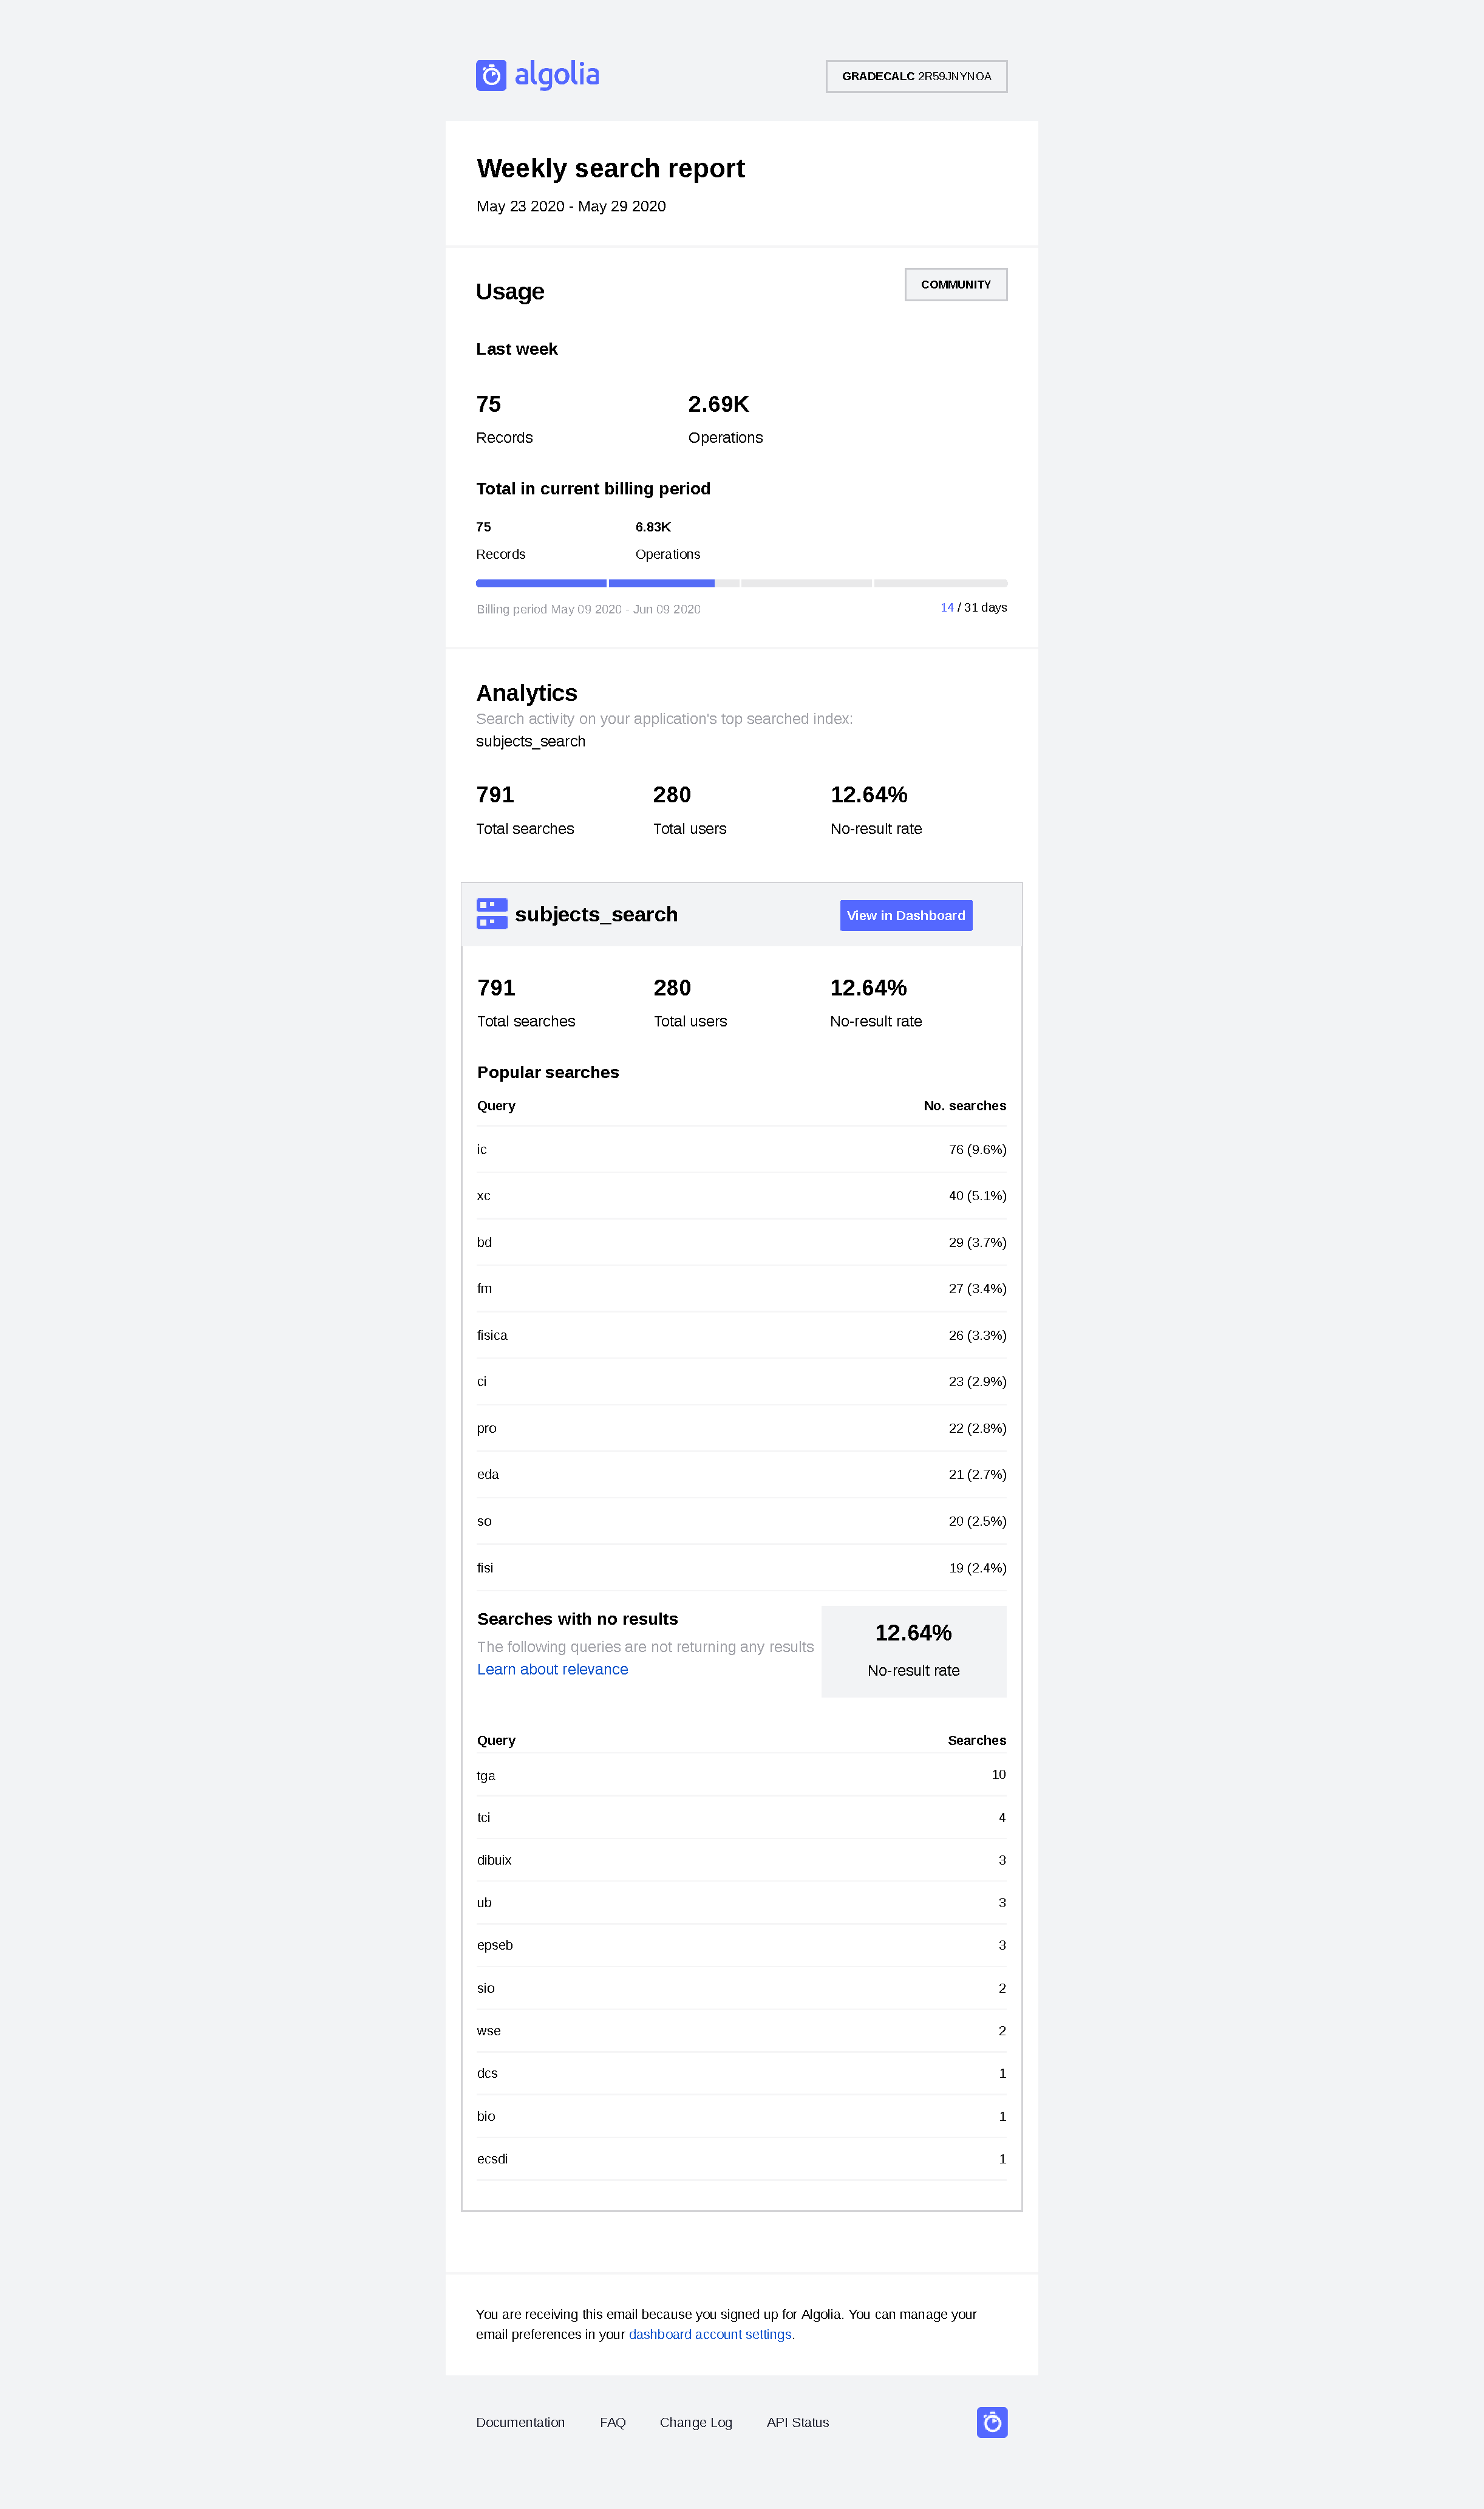
\includegraphics[height=21cm]{media/algolia-email.pdf}
    \caption{Algolia's weekly search report email}
    \label{algolia-email}
\end{figure}
\vfill

\clearpage\newpage
\subsection{Google Analytics}

To analyze GradeCalc's web usage, Google Analytics is used. From time to time I check it to understand the patterns that the visits follow and other information. 

If we observe the visits in figure \ref{fig:analytics}, we can see that there are peaks of activity during the final exam periods. Each time there are more visits. This last semester, there have been fewer visits during the exams period, but users have become more active during non-exam periods.

An \textit{Avg. Session Duration} of 1 minute and 44 seconds is a good number because it means that users engage with the app.

The \textit{bounce rate} is very high, \textit{79.02\%}, but it makes sense and it's not a bad thing in our case. Because the app usual usage happens only in the dashboard, it's normal that users just open one page and leave.

We can see that most of the users, \textit{68.8\%}, are \textit{new visitors}. But on the other hand, approximately one-third of users return.

Finally, half of the visits come from typing the URL in the browser directly. This is a very high value, but it's executable because the app can be installed, meaning that each time a user opens it counts as direct.

\vfill
\begin{figure}[h!]
    \center
    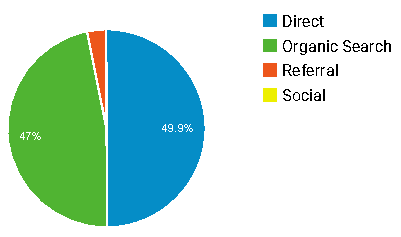
\includegraphics[width=0.5\columnwidth]{media/analytics-acquisition.pdf}
    \caption{Google analytics acquisition sources}
    \label{fig:analytics-acquisition}
\end{figure}
\vfill

\clearpage\newpage\null

\vfill
\begin{figure}[h!]
    \center
    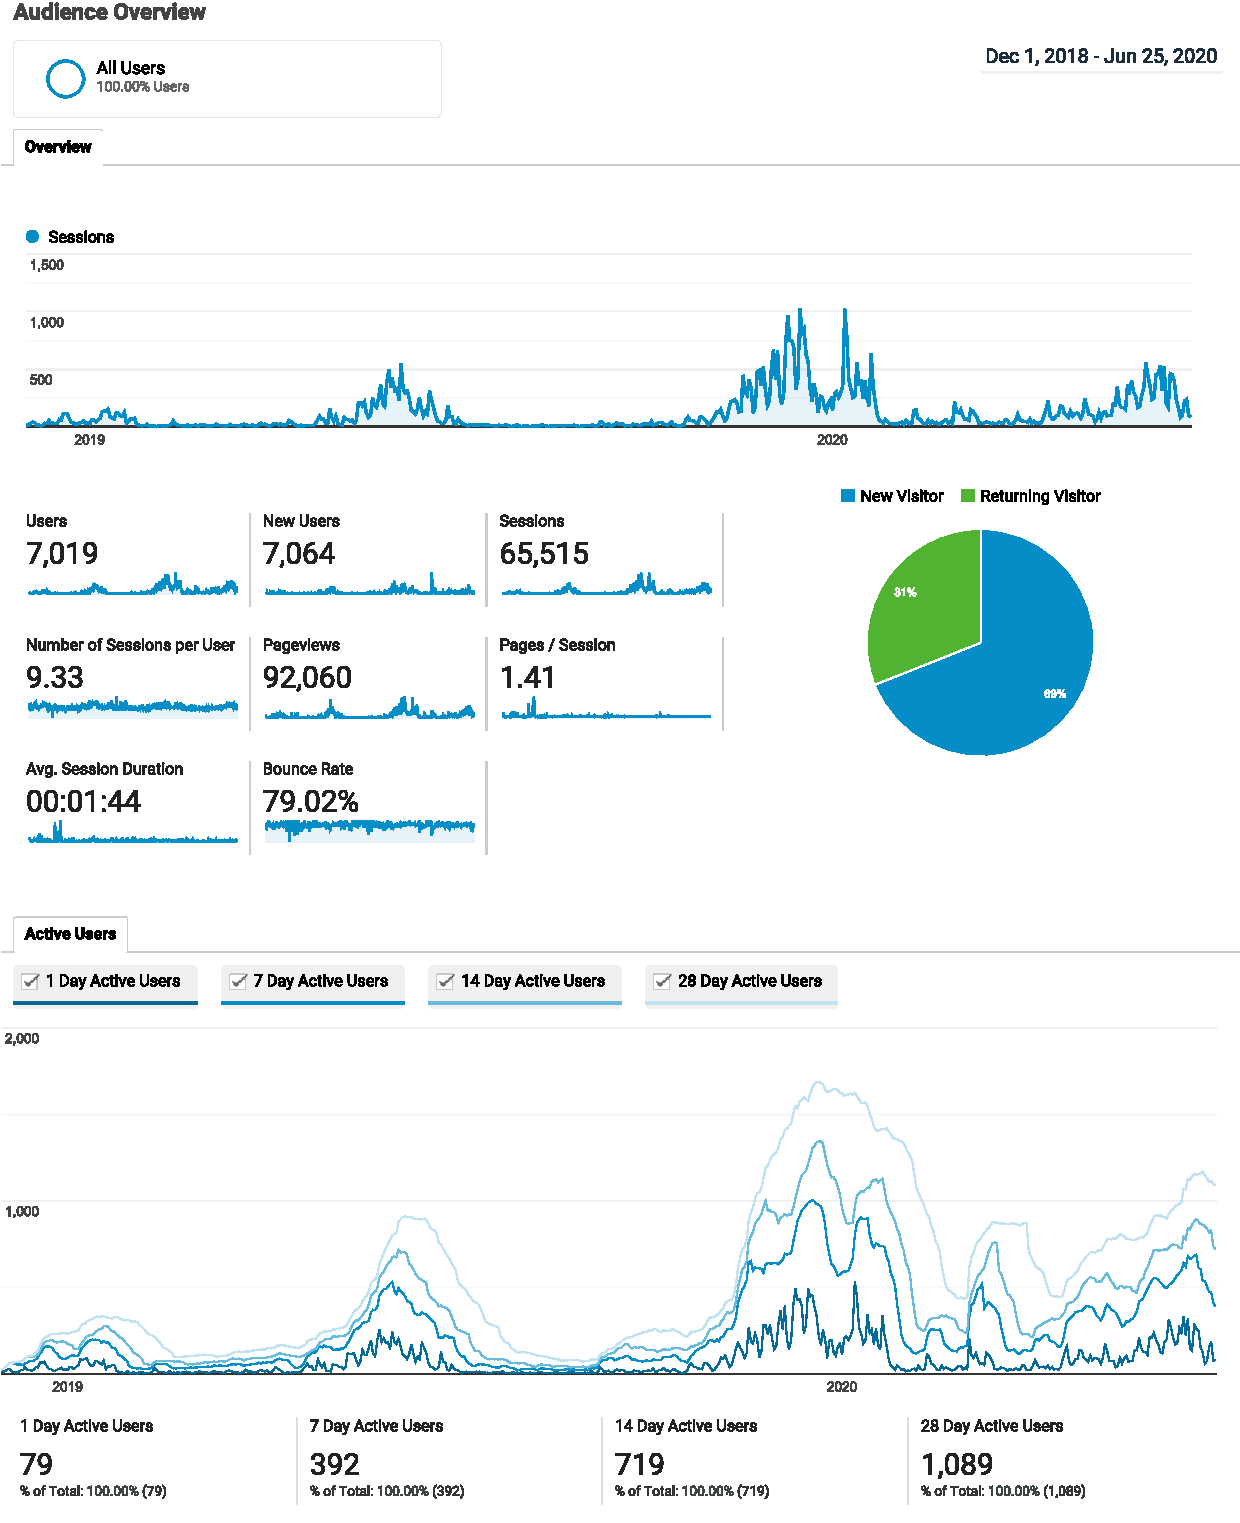
\includegraphics[width=1\columnwidth]{media/analytics-double-report.pdf}
    \caption{Sessions report and Active users report - Google analytics}
    \label{fig:analytics}
\end{figure}
\vfill

\clearpage\newpage
\subsection{Google Search Console}

Finally, to ensure that the app is searchable in Google. The domain is registered in Google Search Console. If there are any crawling errors I'll receive an email. But the typical use of this app is to understand how users find the page. 

In the figure \ref{fig:search-console-queries} we can see that all the queries are combinations of the words \textit{Grade} and \textit{Calc}, in some cases with typos. And there are no queries like \textit{Calculadora notas}, they are highly competitive queries that are not worth fighting for the first place. But if they search \textit{Calculadora notas FIB} or \textit{Calcular notas FIB} the app is in the first result. This second query is more likely to happen, although, as we see, none is searching for it.

\vfill
\begin{figure}[h!]
    \center
    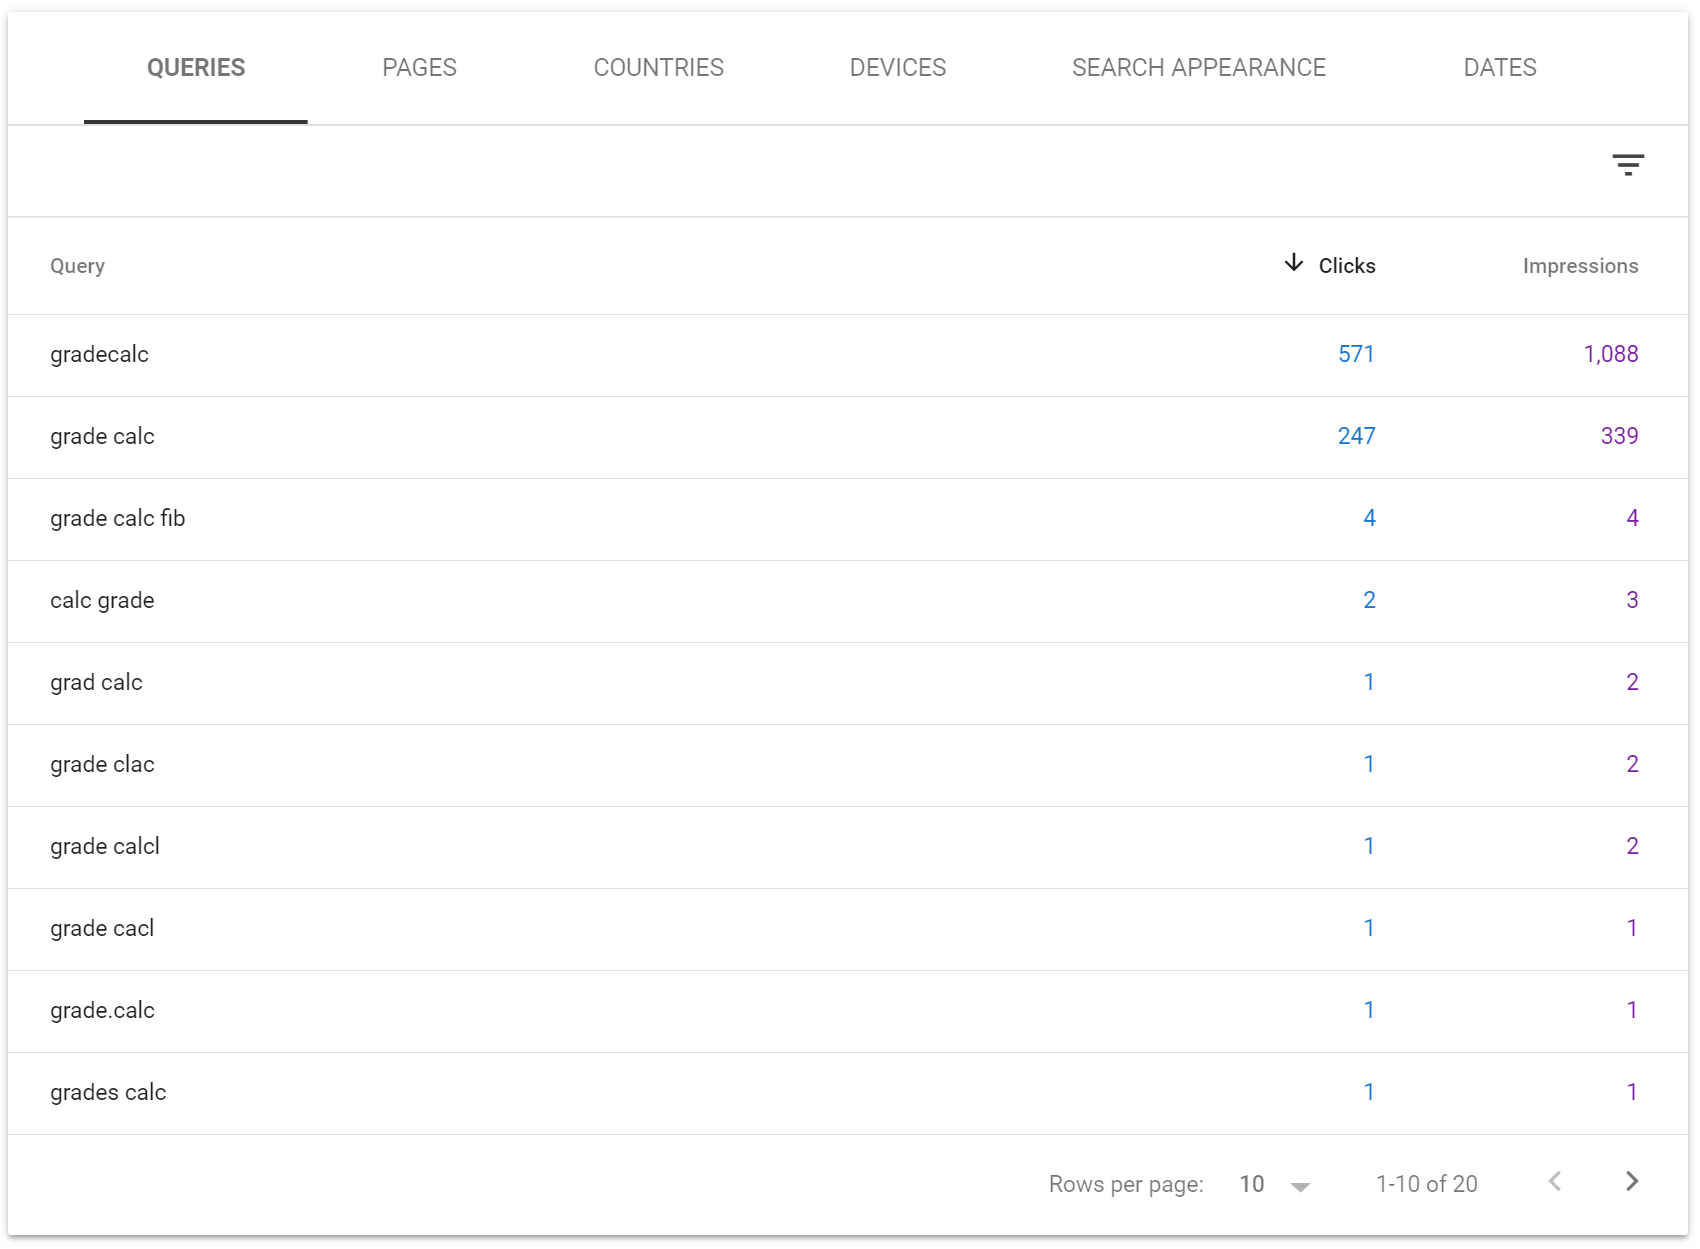
\includegraphics[width=1\columnwidth]{media/search-conole-queries.png}
    \caption{Google search console queries}
    \label{fig:search-console-queries}
\end{figure}
\vfill

\clearpage\newpage\null

\vfill
\begin{figure}[h!]
    \center
    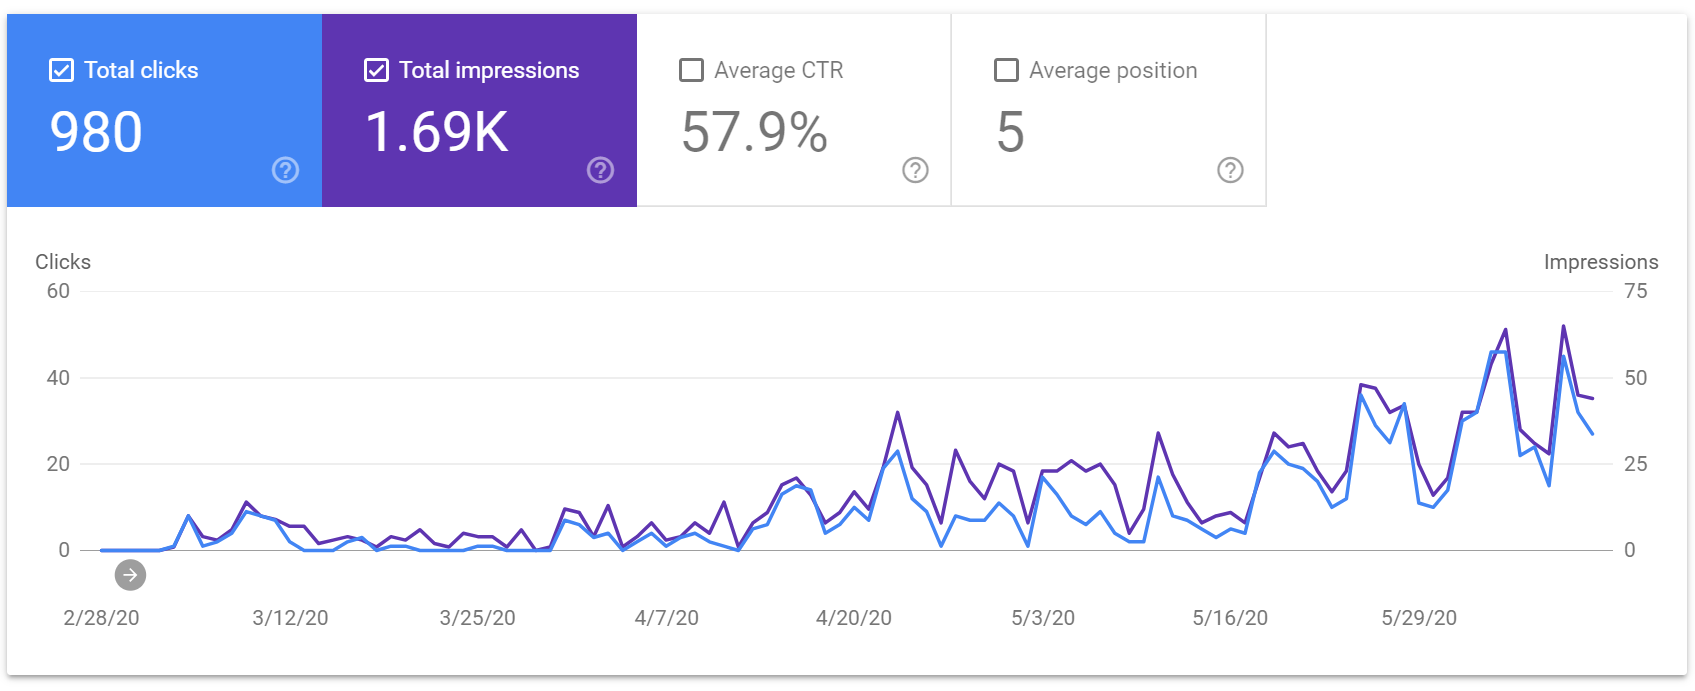
\includegraphics[width=1\columnwidth]{media/search-console-plot.png}
    \caption{Google search console performance}
    \label{fig:search-console-plot}
\end{figure}
\vfill
\begin{figure}[h!]
    \center
    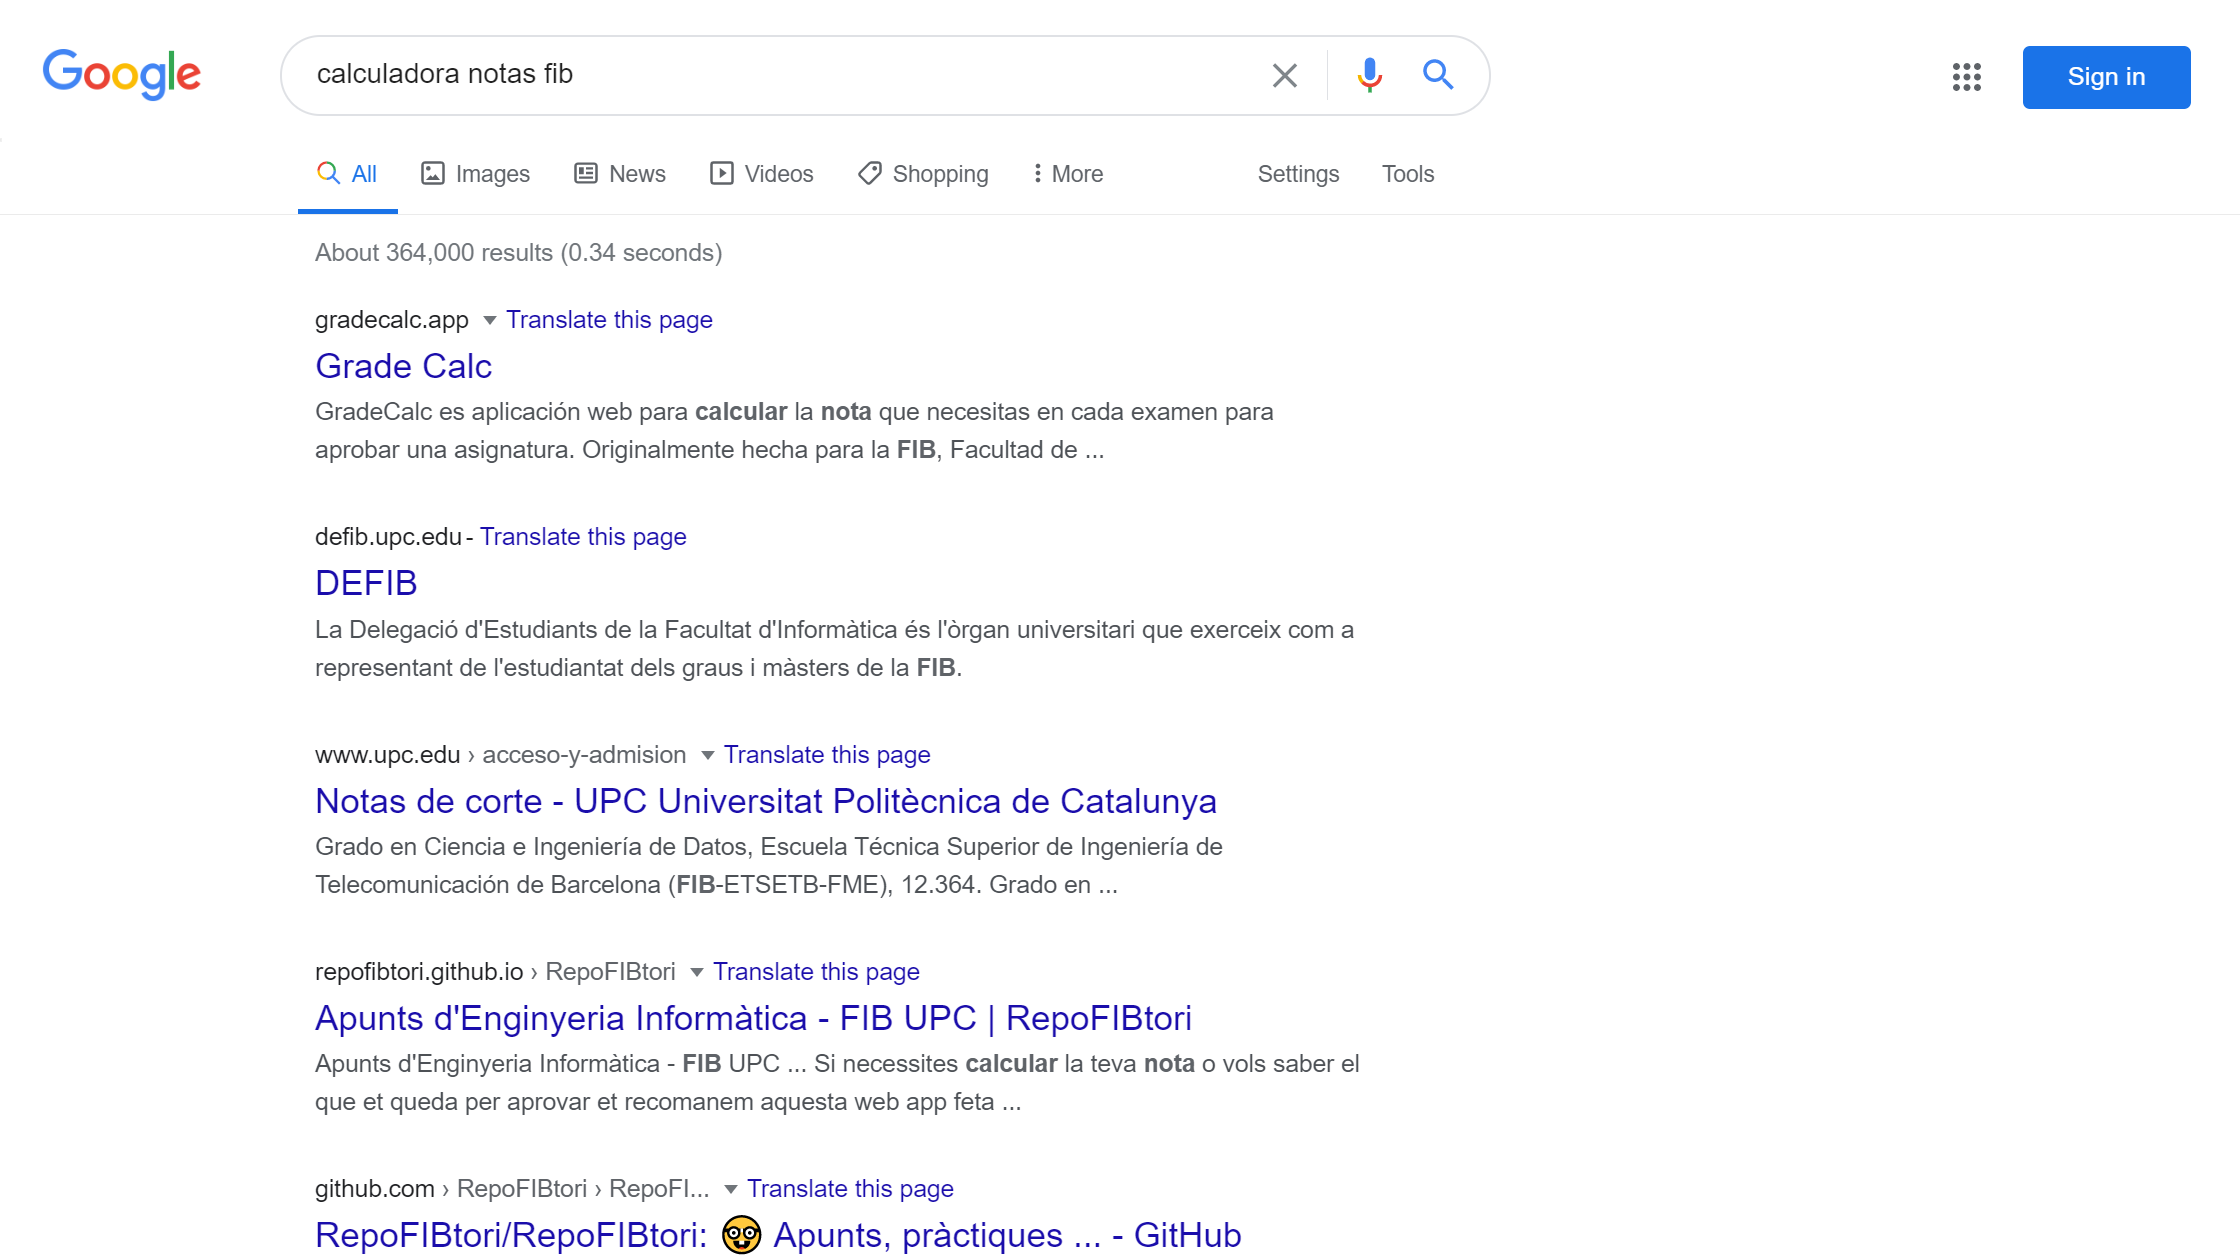
\includegraphics[frame,width=1\columnwidth]{media/screenshot-first-google-result.png}
    \caption{Google result for \textit{Calculadora notas FIB}}
    \label{fig:first-result}
\end{figure}
\vfill

